
\documentclass[%
 reprint,
%superscriptaddress,
%groupedaddress,
%unsortedaddress,
%runinaddress,
%frontmatterverbose, 
%preprint,
%preprintnumbers,
%nofootinbib,
%nobibnotes,
%bibnotes,
 amsmath,amssymb,
 aps,
%pra,
%prb,
%rmp,
%prstab,
%prstper,
%float,
]{revtex4-2}
\usepackage{url}
\usepackage{float}
\usepackage{graphicx}% Include figure files
\usepackage{dcolumn}% Align table columns on decimal point
\usepackage{bm}% bold math
%\usepackage{hyperref}% add hypertext capabilities
%\usepackage[mathlines]{lineno}% Enable numbering of text and display math
%\linenumbers\relax % Commence numbering lines

%\usepackage[showframe,%Uncomment any one of the following lines to test 
%%scale=0.7, marginratio={1:1, 2:3}, ignoreall,% default settings
%%text={7in,10in},centering,
%%margin=1.5in,
%%total={6.5in,8.75in}, top=1.2in, left=0.9in, includefoot,
%%height=10in,a5paper,hmargin={3cm,0.8in},
%]{geometry}

\begin{document}

\preprint{APS/123-QED}

\title{Measurement of the Speed of Light in Air with Laser Pulses}% Force line breaks with \\

\author{Dean Reiter}
\affiliation{%
 Cornell University\\
}%

\date{\today}% It is always \today, today,
             %  but any date may be explicitly specified

\begin{abstract}
An experimental measurement of the speed of light in air is presented. [Background?] [Experiment] [Analysis Method] [Result]

\end{abstract}

%\keywords{Suggested keywords}%Use showkeys class option if keyword
                              %display desired
\maketitle

%\tableofcontents

\section{Introduction}

[Historical Background]

[Physics]

\section{Experimental Setup}

The optical setup pictured in Fig. 1 is similar to a Michelson interferometer, but it is not used to measure an interference pattern. The red laser used is similar to a commercial, low-power laser pointer, and its effective power is reduced to 0.56 mW by a polarizing filter, which is not shown in Fig. 1. The laser beam travels 20 cm before passing through a beam splitter. One of the split beams travels a short path, passing through another polarizing filter (not shown in Fig. 1) and reflecting off a mirror, which is 19.50 $\pm$ 0.25 cm away, before returning to the beam splitter. The other split beam travels a long path, reflecting off a parabolic mirror, which is 10.490 $\pm$ 0.101 m away from the beam splitter, and four times between that mirror and another, which is a distance of 10.235 $\pm$ 0.101 m from the first, before finally returning to the beam splitter. The redirected beams travel a final 37 cm before entering a photomultiplier tube. The overall path length difference $\Delta x$ between the long and short paths is 102.47 $\pm$ 1.02 m. 

\begin{figure}[H]
\centering
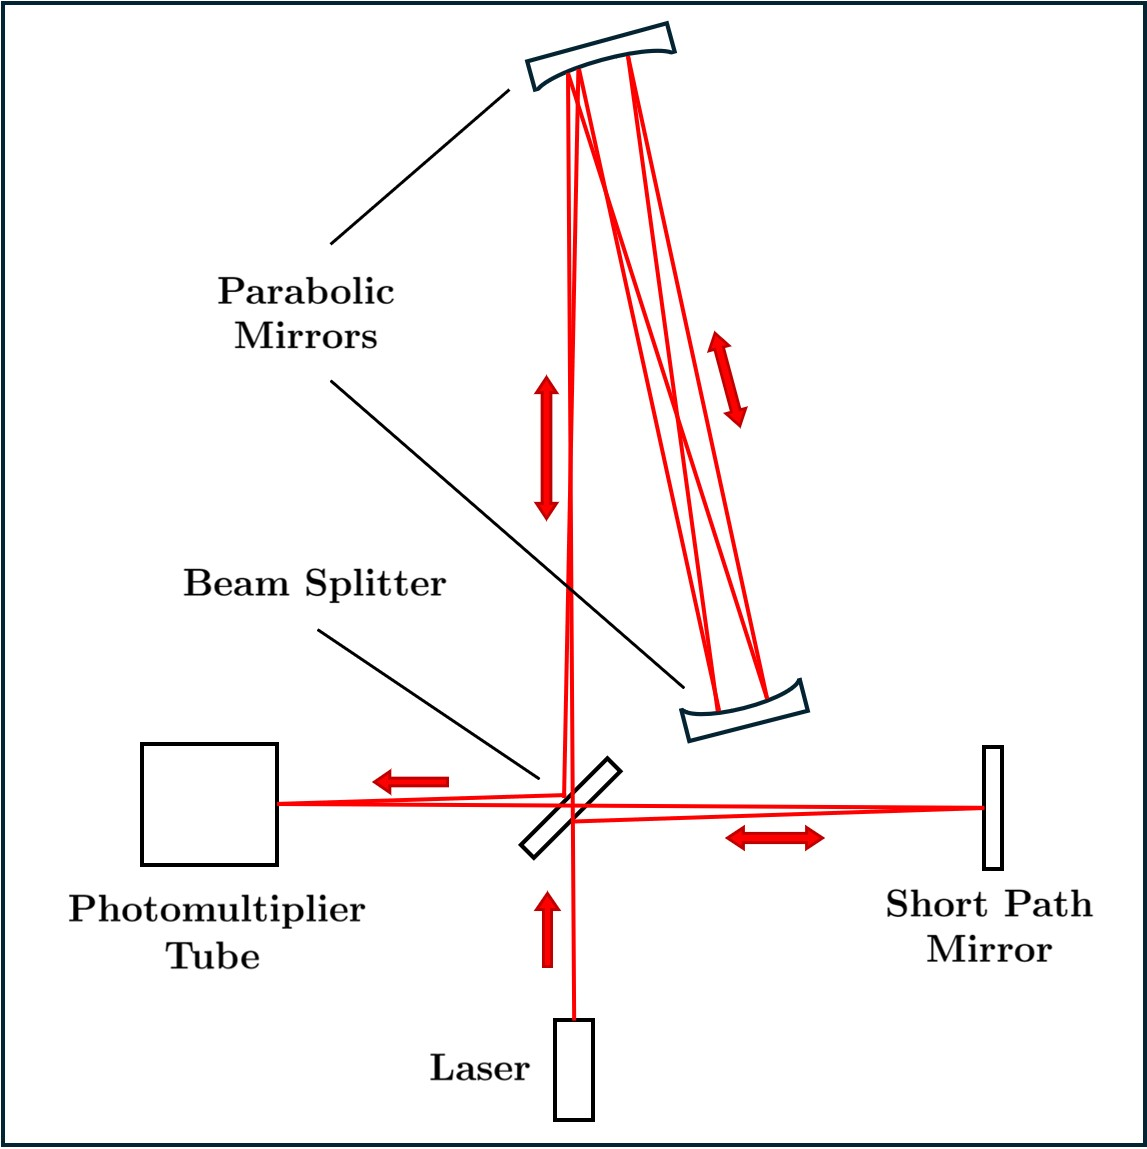
\includegraphics[width=0.75\columnwidth]{Diagram.jpg}% Here is how to import EPS art
\caption{\label{fig:epsart} Optical setup in which a laser beam is split into two paths. The beam traveling the long path reflects five times between parabolic mirrors positioned 10 meters away before returning to the beam splitter, resulting in a total path length that is 102.45 $\pm$ 1.02 m longer than that of the beam which travels the short path. The split paths are recombined and directed to a photomultiplier which measures light intensity.}
\end{figure}

The electronic equipment consists of a high-voltage DC power supply, a photomultiplier tube, a voltage amplifier, a Systron Donner 101 Pulse Generator, and a Tektronix TBS 2000B Series Digital Oscilloscope. The photomultiplier tube, which is given a 900 V supply, produces an electrical current when it detects photons from the laser beam. The photomultiplier output is amplified by 50 dB and measured by the oscilloscope. The pulse generator supplies the laser with square-wave voltage pulses with a width of 3.0 $\pm$ 0.1 $\mu$s at a frequency of 1.0 kHz. This is the shortest pulse width that can activate the laser diode, which is not designed to be pulsed for extremely short durations. A reference signal from the pulse generator, which is proportional to the signal it supplies the laser, triggers the oscilloscope. Since the photomultiplier output is highly sensitive, the oscilloscope records the average of 512 trigger cycles of the photomultiplier signal to reduce noise.

The optical setup was adjusted to perform measurements of the long-path and short-path beams individually. An opaque plate was positioned to obstruct either the short path or the long path as desired to measure the beam which travels each path in isolation. Due to the unknown time-dependence of the photomultiplier and amplifier's electrical response to light intensity, the polarizing filter between the beam splitter and short path mirror (not shown in Fig. 1) was calibrated so that the difference between the average signal amplitude of the short and long-path beams is less than 50 mV.

\section{Data and Analysis}

The intensities as a function of time of the laser beam pulses which travel the two paths in the optical setup in Fig. 1 were measured by a photomultiplier. The intensities of the long-path and short-path beams were each measured in isolation by individually obstructing the beam paths. The amplified laser pulse signals produced by the photomultiplier were averaged over 512 pulse cycles of 1 kHz and recorded by an oscilloscope. Each waveform recording contains 20 thousand averaged measurements of the voltage of the amplified photomultiplier signal over a duration of 20 $\mu$s. The averages of 10 oscilloscope recordings of each laser pulse signal are shown in Fig. 2. 

\begin{figure}[H]
\centering
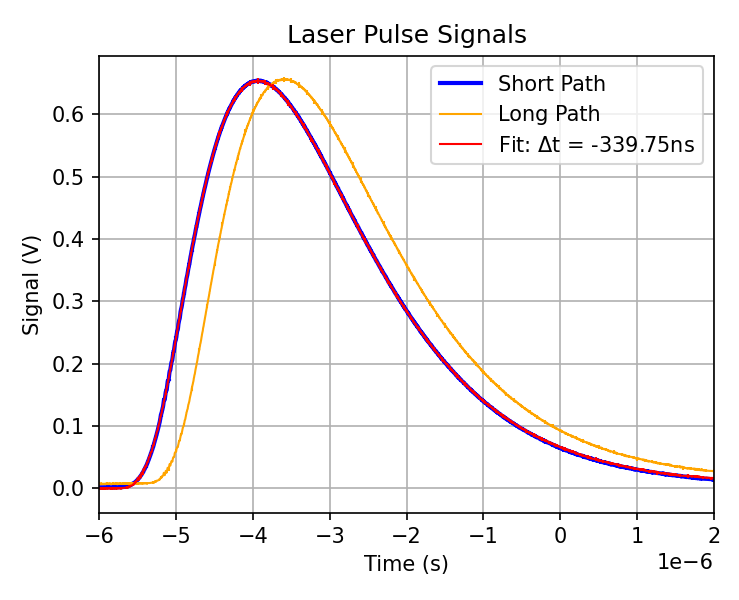
\includegraphics[width=0.9\columnwidth]{Signals2.png}% 
\caption{\label{fig:epsart} An 8 $\mu$s selection of the averaged electrical signals produced by laser pulses which traveled the long path (yellow) and by those which traveled the short path (blue) in the apparatus in Fig. 1. The long-path signal is advanced by 339.75 ns and fitted to the short-path signal (red). Each signal shown is the average of 5,120 pulses. The error bars shown are too small to distinguish. }
\end{figure}

 A non-linear least squares minimization is used to fit the averaged long-path signal to the averaged short-path signal. The fitted data is shown in red in Fig. 2. The timescale of the oscilloscope data, which is triggered by the pulse generator at 1 kHz, is used as an objective timescale by which to compare the long-path and short-path signals. The first and last 0.5 $\mu$s of the short-path signal data is cut, and we define this set of time and voltage measurements as $(t_i, y_i)$. The fitting function $f(t, \vec{\theta})$ with fitting parameters $\vec{\theta} = (a,b,\delta)$ is linearly interpolated from the long-path signal data, which we define as the set $(t_i, x_i)$. 

\begin{figure}[H]
\centering
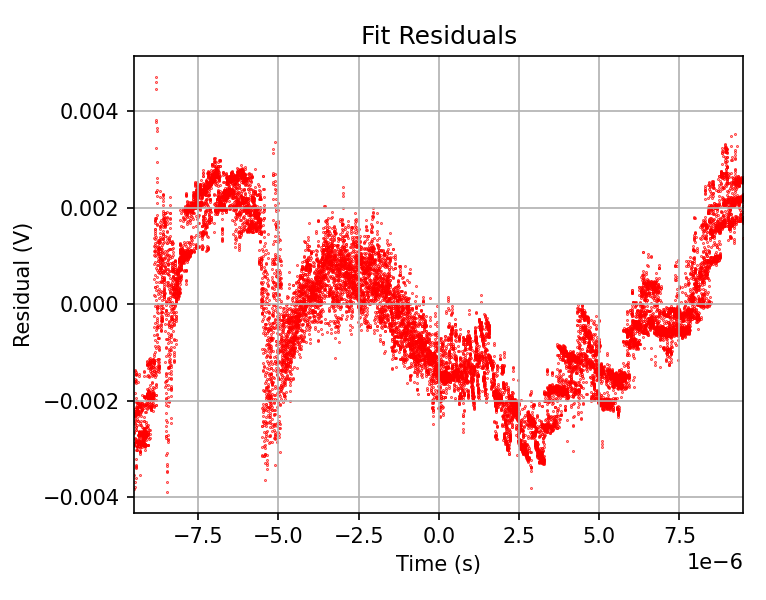
\includegraphics[width=0.9\columnwidth]{Residuals.png}% 
\caption{\label{fig:epsart} FITTING RESIDUALS?}
\end{figure}

[Results]







\section{Conclusion}

[Interpretation of Results]

[Error Analysis]

[Takeaways]

\begin{acknowledgments}

[Acknowledgements]

\end{acknowledgments}


\appendix


\bibliography{main}% Produces the bibliography via BibTeX.

\end{document}
%
% ****** End of file apssamp.tex ******
